\section{First Section}
\begin{frame}{Autenticazione}
  Decidim supporta la gestione dei permessi per i singoli componenti/fasi

  Una di queste prende il nome di \emph{Verifica delle autorizzazioni}

  \begin{wrapfigure}{r}{0.50\textwidth}
    \centering
    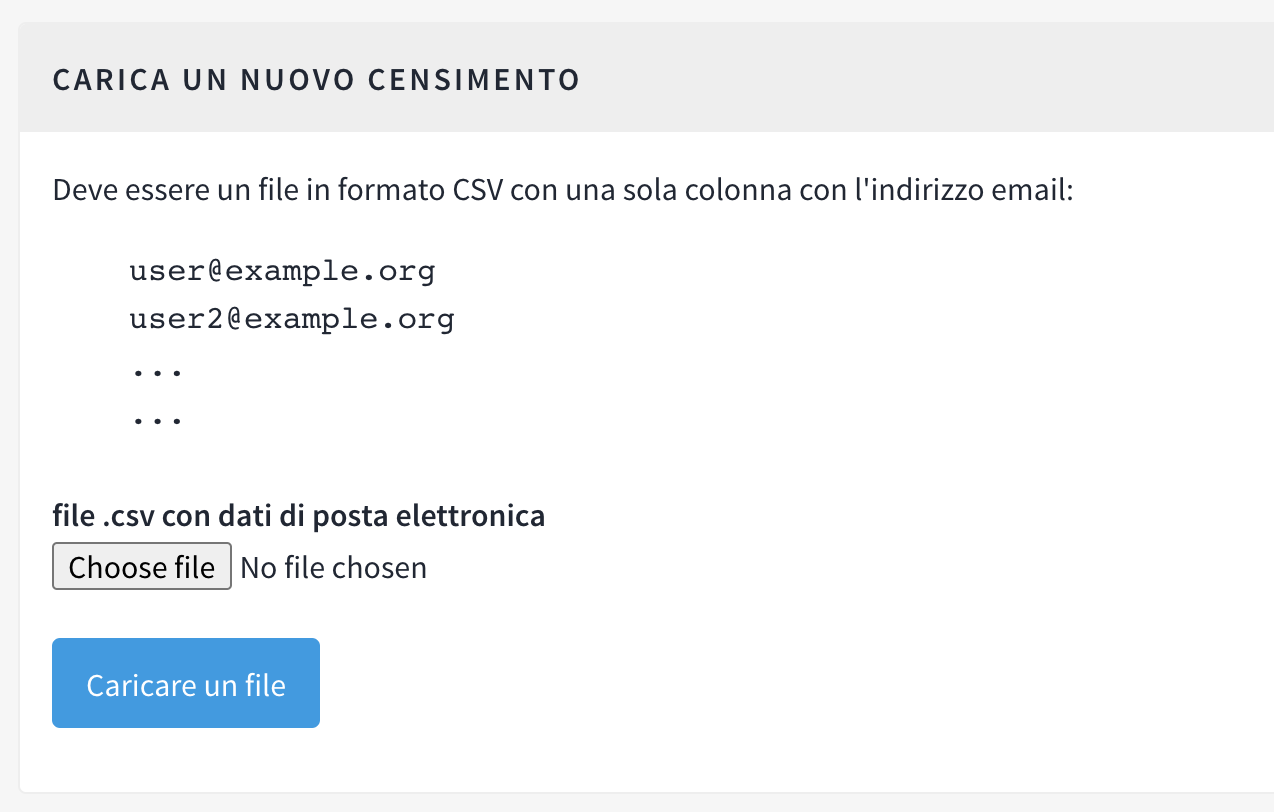
\includegraphics[width=0.50\textwidth]{images/auth}
  \end{wrapfigure}

  Per gestire l'autenticazione si potrebbe importare all'interno di decidim una lista di mail possedute dall'azienda.

  (ad esempio quelle registrate all'interno degli "sportelli" online dell'azienda e quindi validate)

\end{frame}